\documentclass[11pt,a4paper]{ltjsarticle}
\usepackage{graphicx}
\usepackage{amsmath,amssymb}
\usepackage{booktabs}
\usepackage{listings}
\usepackage{xcolor}
\usepackage{float}

% ソースコードの表示設定
\lstset{
    basicstyle=\ttfamily\small,
    commentstyle=\color{green!50!black},
    keywordstyle=\color{blue},
    stringstyle=\color{red},
    showstringspaces=false,
    frame=single,
    numbers=left,
    stepnumber=1
}

\title{第5週 演習課題レポート}
\author{学籍番号: 24RB1074 \and 氏名: 半田悠人}
\date{\today}

\begin{document}
\maketitle

\section{課題1: 最急降下・Newton・BFGSを自作実装}
対象関数: $f(x_{1},x_{2})=x_{1}^{2}+10x_{2}^{2}$, 初期値: $x_{0}=(3,2)$

\subsection{実行結果表}
% プログラムの出力結果
\begin{table}[hbtp]
    \centering
    \caption{各手法の実行結果}
    \begin{tabular}{lcccc}
        \toprule
        手法 & 最終解 $x^*$ & 目的関数値 $f(x^*)$ & 反復回数 & 最終勾配ノルム \\
        \midrule
        最急降下法 & ($3.41 \times 10^{-7}$, $-3.27 \times 10^{-8}$) & $1.27 \times 10^{-13}$ & 63 & $9.45 \times 10^{-7}$ \\
        Newton法  & (0, 0) & 0 & 1 & 0 \\
        BFGS法    & ($1.18 \times 10^{-8}$, $-1.10 \times 10^{-10}$) & $1.39 \times 10^{-16}$ & 6 & $2.37 \times 10^{-8}$ \\
        \bottomrule
    \end{tabular}
\end{table}

\subsection{収束経路の図}
\begin{figure}[H]
    \centering
    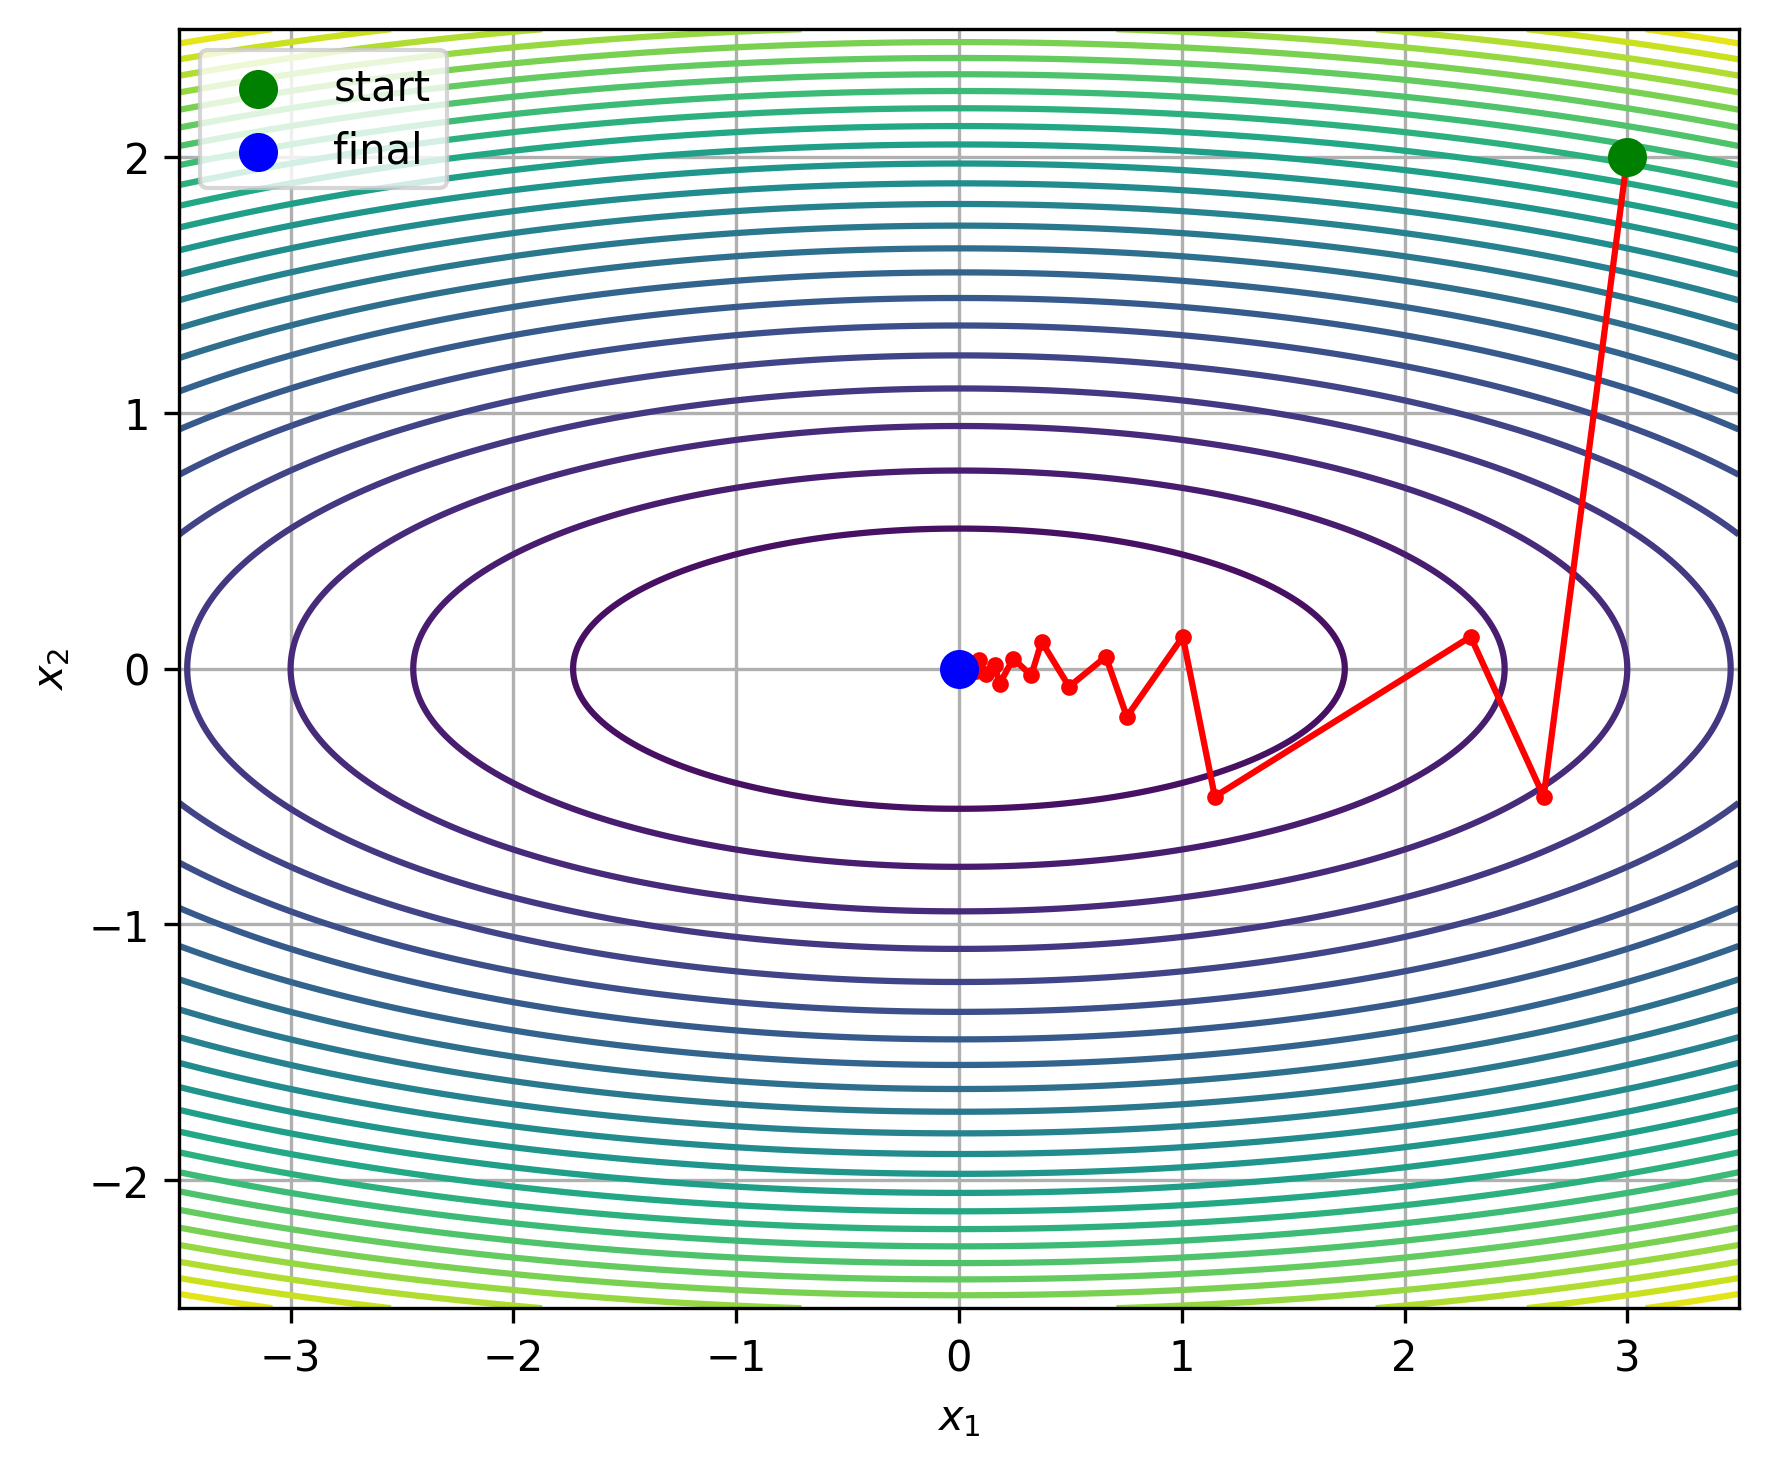
\includegraphics[width=8.5cm]{plots/kadai1_最急降下法.png}
    \caption{最急降下法の収束経路}
    \label{fig:task1_gradient}
\end{figure}

\begin{figure}[H]
    \centering
    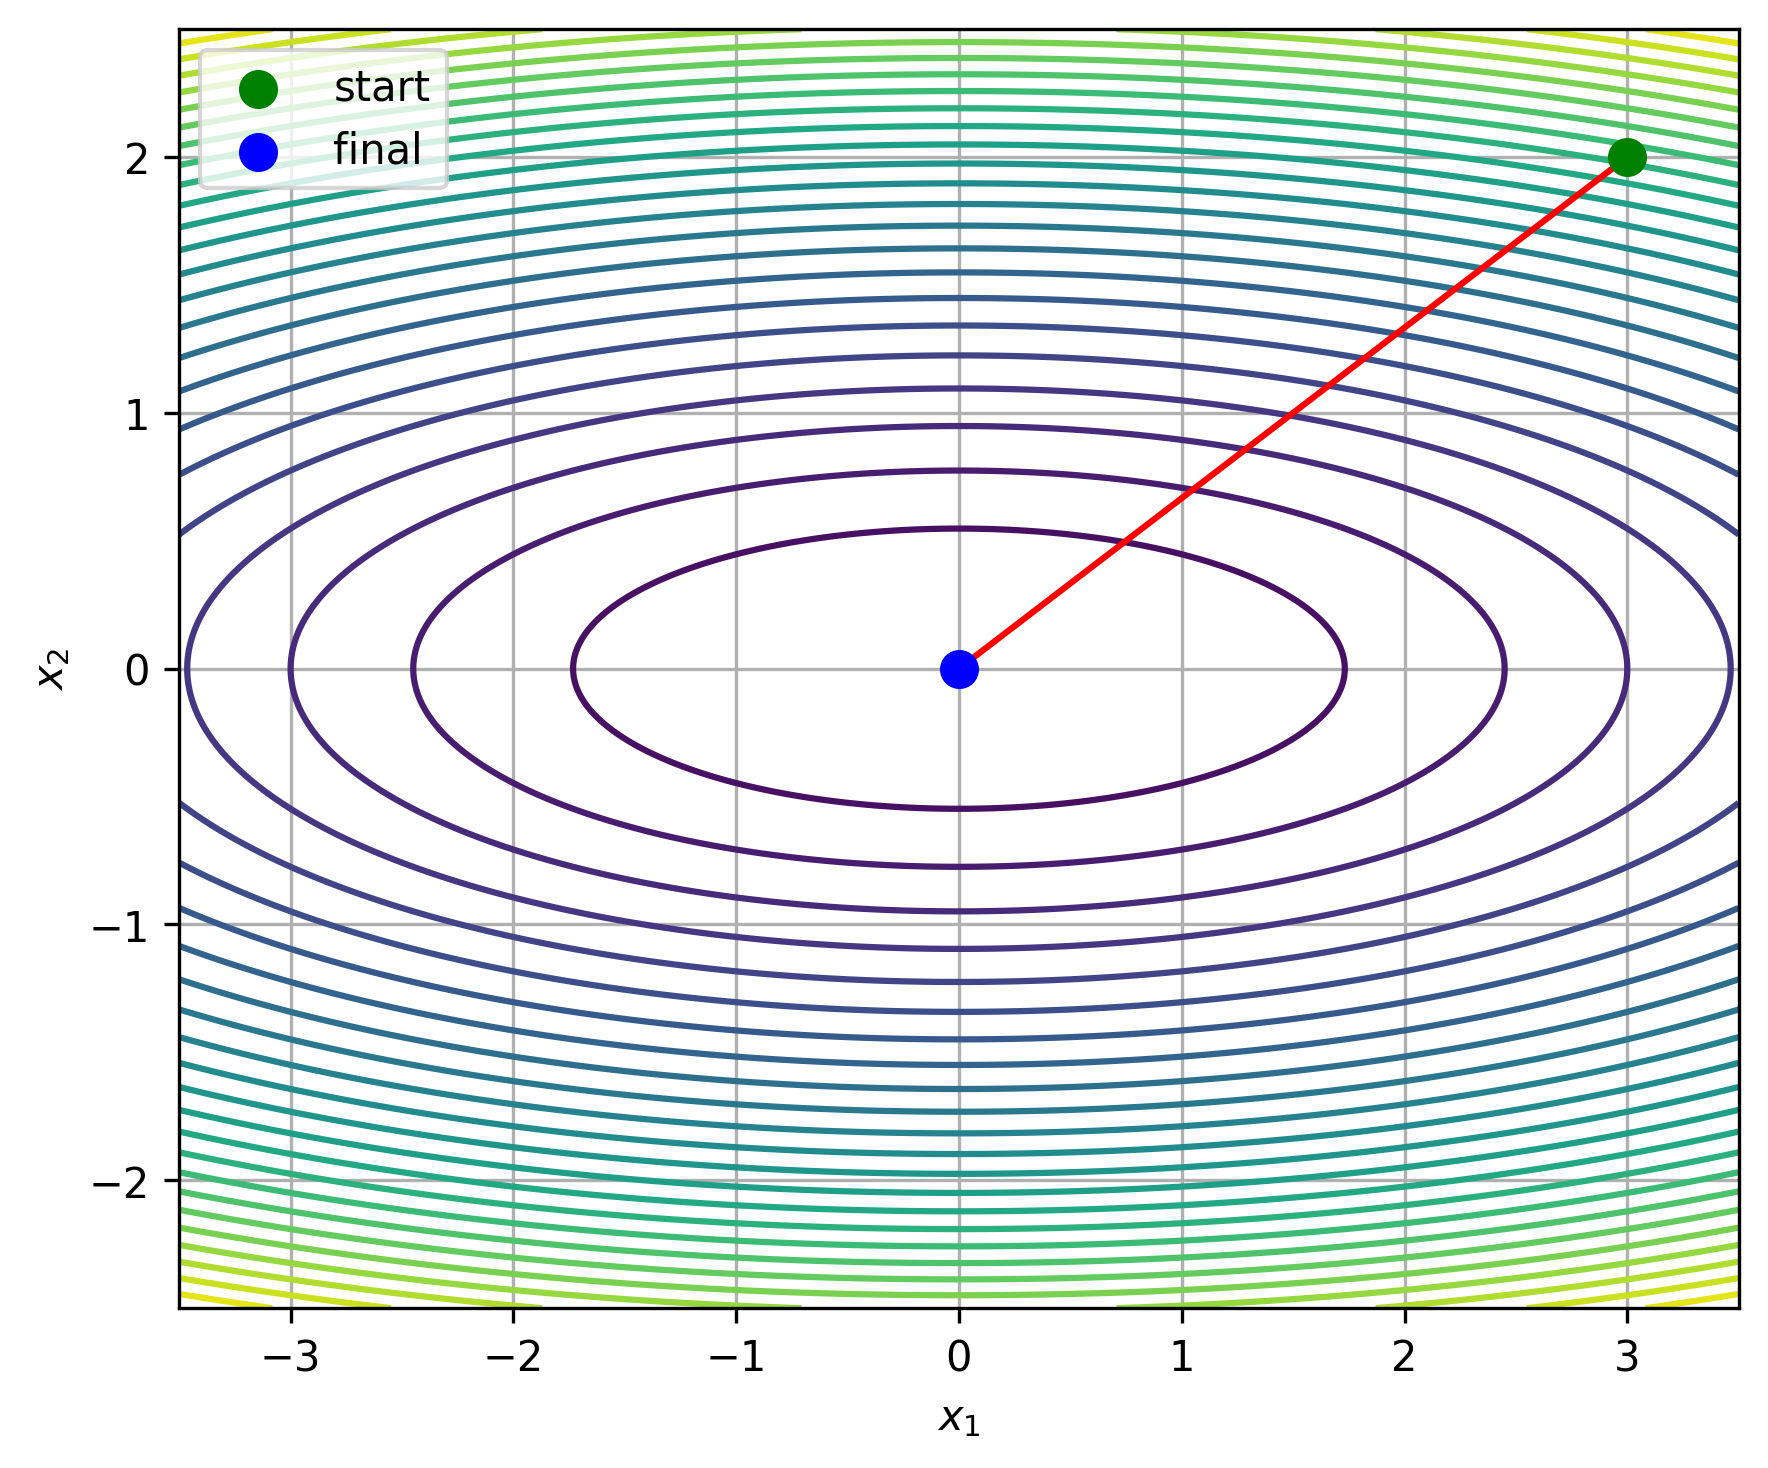
\includegraphics[width=8.5cm]{plots/kadai1_Newton法.png}
    \caption{Newton法の収束経路}
    \label{fig:task1_newton}
\end{figure}

\begin{figure}[H]
    \centering
    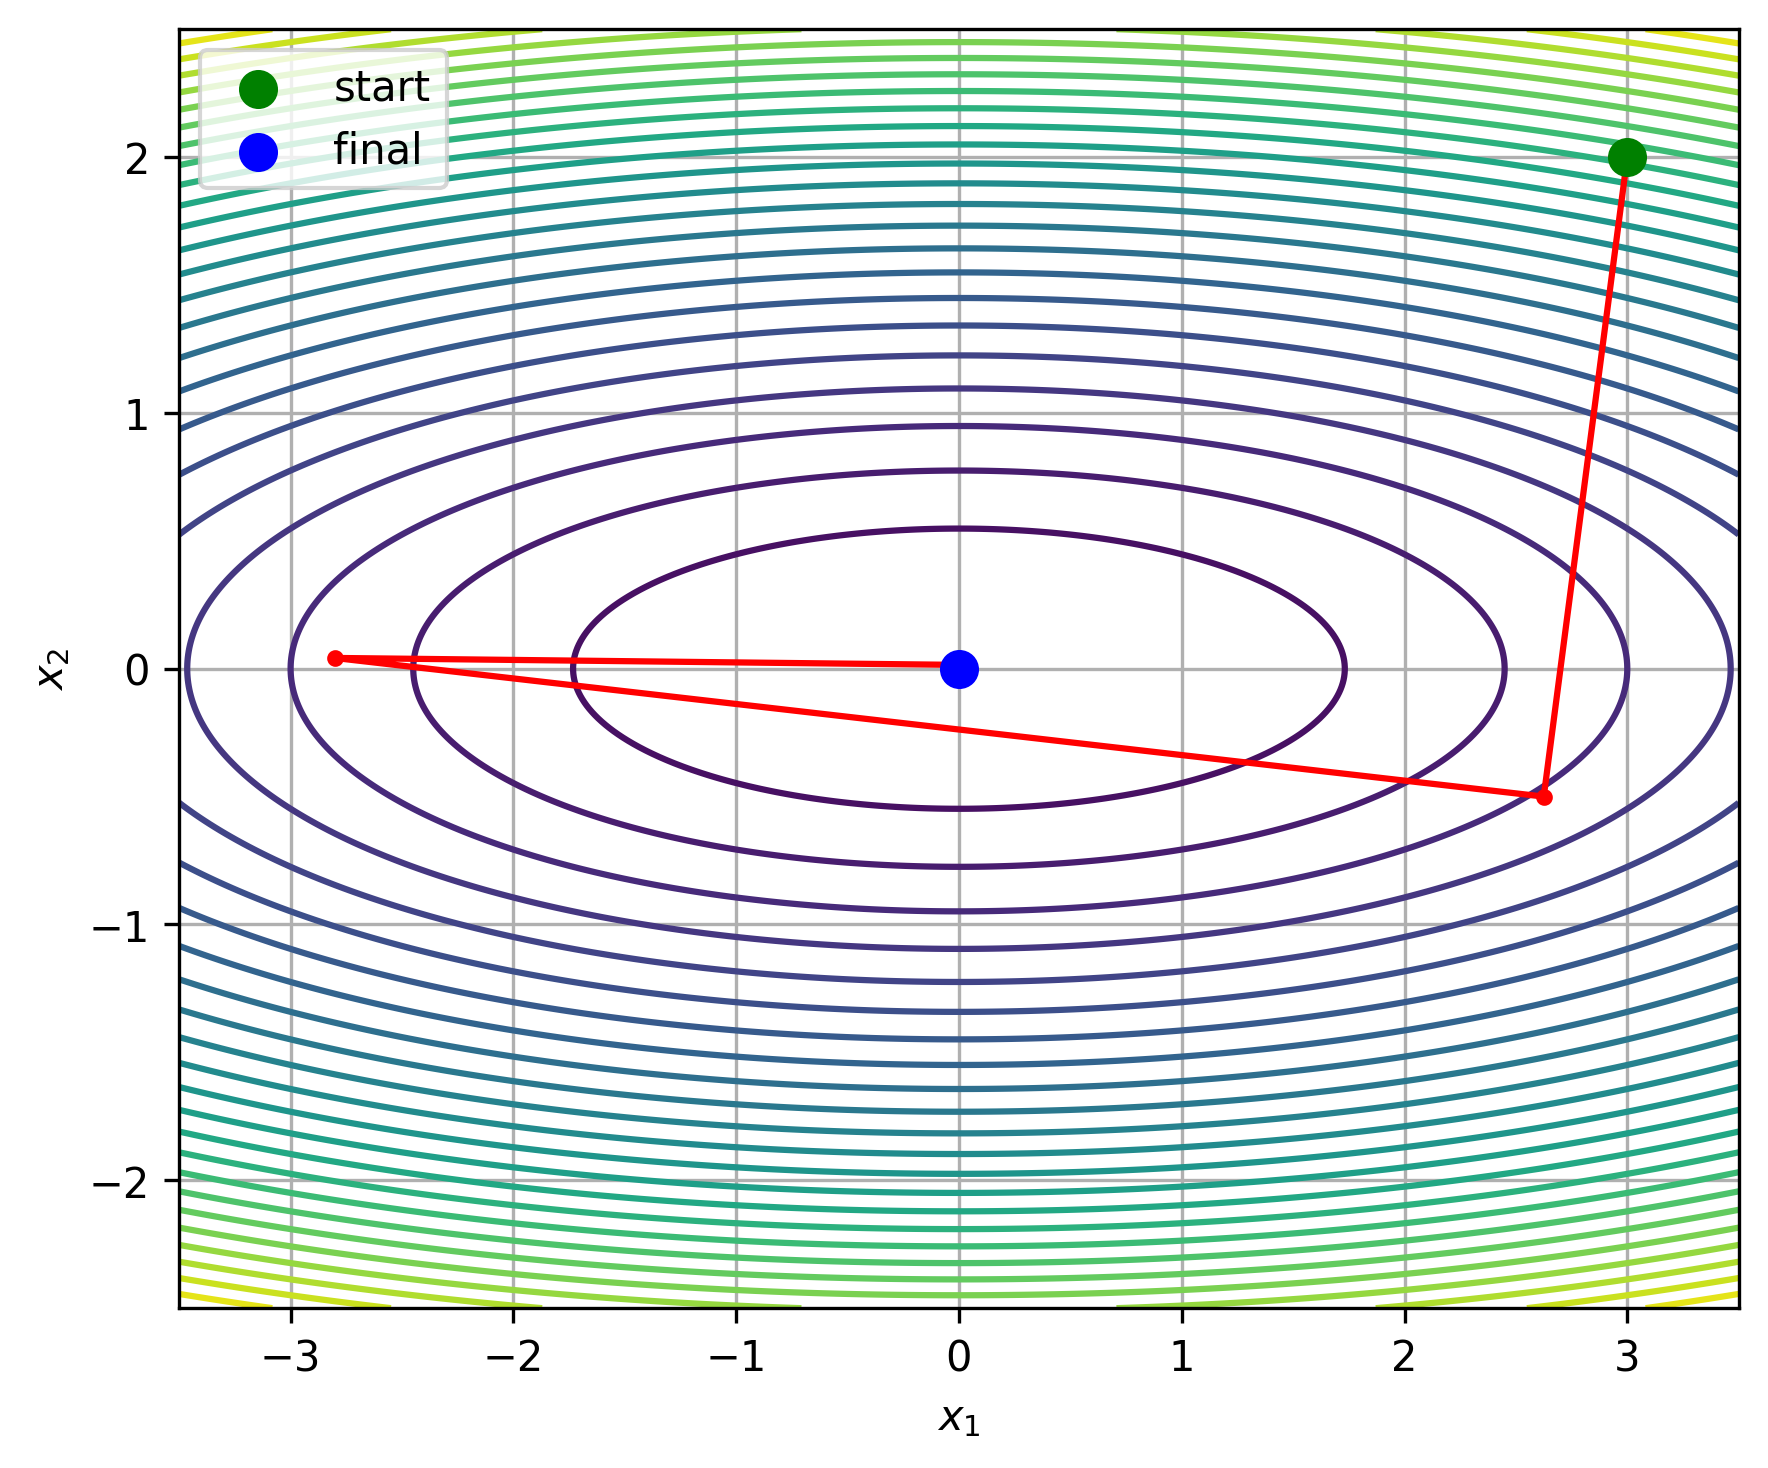
\includegraphics[width=8.5cm]{plots/kadai1_BFGS法.png}
    \caption{BFGS法の収束経路}
    \label{fig:task1_bfgs}
\end{figure}

\subsection{考察}
3手法は同じ停止条件 $\|\nabla f(x_k)\|<10^{-6}$ または最大反復回数への到達を用いたが、
反復回数には大きな差が生じた。最急降下法は63回を要し、図\ref{fig:task1_gradient}では
収束経路が谷を横切るようにジグザグしている。本問のHesse行列は
$\nabla^2 f=\mathrm{diag}(2,20)$ であり、$x_1$方向と$x_2$方向で曲率が10倍異なる。
そのため、負の勾配方向は最適解を直接向かず、直線探索で刻み幅を調整しながら少しずつ収束したと考えられる。
最急降下法はHesse行列を必要とせず、一般に1反復当たりの記憶量と計算量が小さい一方、
曲率の差が大きい問題では反復回数が増えやすい。

Newton法は1回の更新で厳密解 $(0,0)$ に到達した。本問は二次関数でHesse行列が一定であるため、
Newton方向 $d_k=-(\nabla^2 f)^{-1}\nabla f(x_k)$ が初期点から最適解への方向と一致するからである。
ただし、$n$変数の一般問題ではHesse行列の計算・保存に加え、連立一次方程式の求解に
おおむね $O(n^3)$ の計算量と $O(n^2)$ の記憶量を要する。このため、本問のような小規模問題では非常に有効であるが、
大規模問題では1反復の負担が大きくなる。

BFGS法は6回で収束し、最急降下法より大幅に少ない反復回数で、Hesse行列を解析的に与えたNewton法に近い収束性能を示した。
BFGS法は勾配の変化からHesse行列を逐次近似するため、初期反復では近似が不十分であるものの、
更新を重ねるにつれて曲率情報を捉え、ジグザグを抑えられたと考えられる。
一方で、近似行列の保存と更新には $O(n^2)$ の記憶量・計算量が必要であり、
今回の実装ではさらに各反復で連立一次方程式を解いている。
以上より、1反復の軽さでは最急降下法、反復回数ではNewton法が優れ、BFGS法はHesse行列を直接計算せずに
両者の中間的な計算コストで高い収束性を得る手法であるといえる。

\clearpage
\section{課題2: 初期値によって異なる解に収束することを体験}
Himmelblau関数: $f(x,y)=(x^{2}+y-11)^{2}+(x+y^{2}-7)^{2}$

\subsection{実行結果表}
\begin{table}[hbtp]
    \centering
    \caption{Himmelblau関数における初期値依存性の結果}
    \begin{tabular}{cllccc}
        \toprule
        初期値 & 手法 & 最終解 $x^*$ & $f(x^*)$ & 反復回数 & 収束先番号 \\
        \midrule
        $(-4, 4)$ 
        & 最急降下法 & (3.58, -1.85)  & $3.35 \times 10^{-15}$ & 40 & 4 \\
        & Newton法  & (-2.81, 3.13)  & $1.34 \times 10^{-22}$ & 5 & 2 \\
        & BFGS法    & (3.58, -1.85)  & $8.41 \times 10^{-21}$ & 12 & 4 \\
        \midrule
        $(-3, -3)$ 
        & 最急降下法 & (-3.78, -3.28) & $4.27 \times 10^{-17}$ & 14 & 3 \\
        & Newton法  & (-3.78, -3.28) & $3.34 \times 10^{-22}$ & 5 & 3 \\
        & BFGS法    & (-3.78, -3.28) & $4.83 \times 10^{-19}$ & 9 & 3 \\
        \midrule
        $(0, 0)$ 
        & 最急降下法 & (3.00, 2.00)   & $8.19 \times 10^{-16}$ & 25 & 1 \\
        & Newton法  & ($-3.50 \times 10^{-16}$, $-8.88 \times 10^{-16}$) & 170.00 & 100 & 未収束（上限到達） \\
        & BFGS法    & (3.00, 2.00)   & $1.43 \times 10^{-19}$ & 10 & 1 \\
        \midrule
        $(3, 3)$ 
        & 最急降下法 & (3.00, 2.00)   & $4.91 \times 10^{-15}$ & 21 & 1 \\
        & Newton法  & (3.00, 2.00)   & $1.12 \times 10^{-19}$ & 5 & 1 \\
        & BFGS法    & (3.00, 2.00)   & $5.54 \times 10^{-18}$ & 8  & 1 \\
        \midrule
        $(5, -2)$ 
        & 最急降下法 & (-3.78, -3.28) & $3.71 \times 10^{-16}$ & 13 & 3 \\
        & Newton法  & (3.58, -1.85)  & $5.14 \times 10^{-24}$ & 5 & 4 \\
        & BFGS法    & (-3.78, -3.28) & $3.52 \times 10^{-15}$ & 11 & 3 \\
        \bottomrule
    \end{tabular}
\end{table}

\clearpage
\subsection{収束経路の図}
\begin{figure}[H]
    \centering
    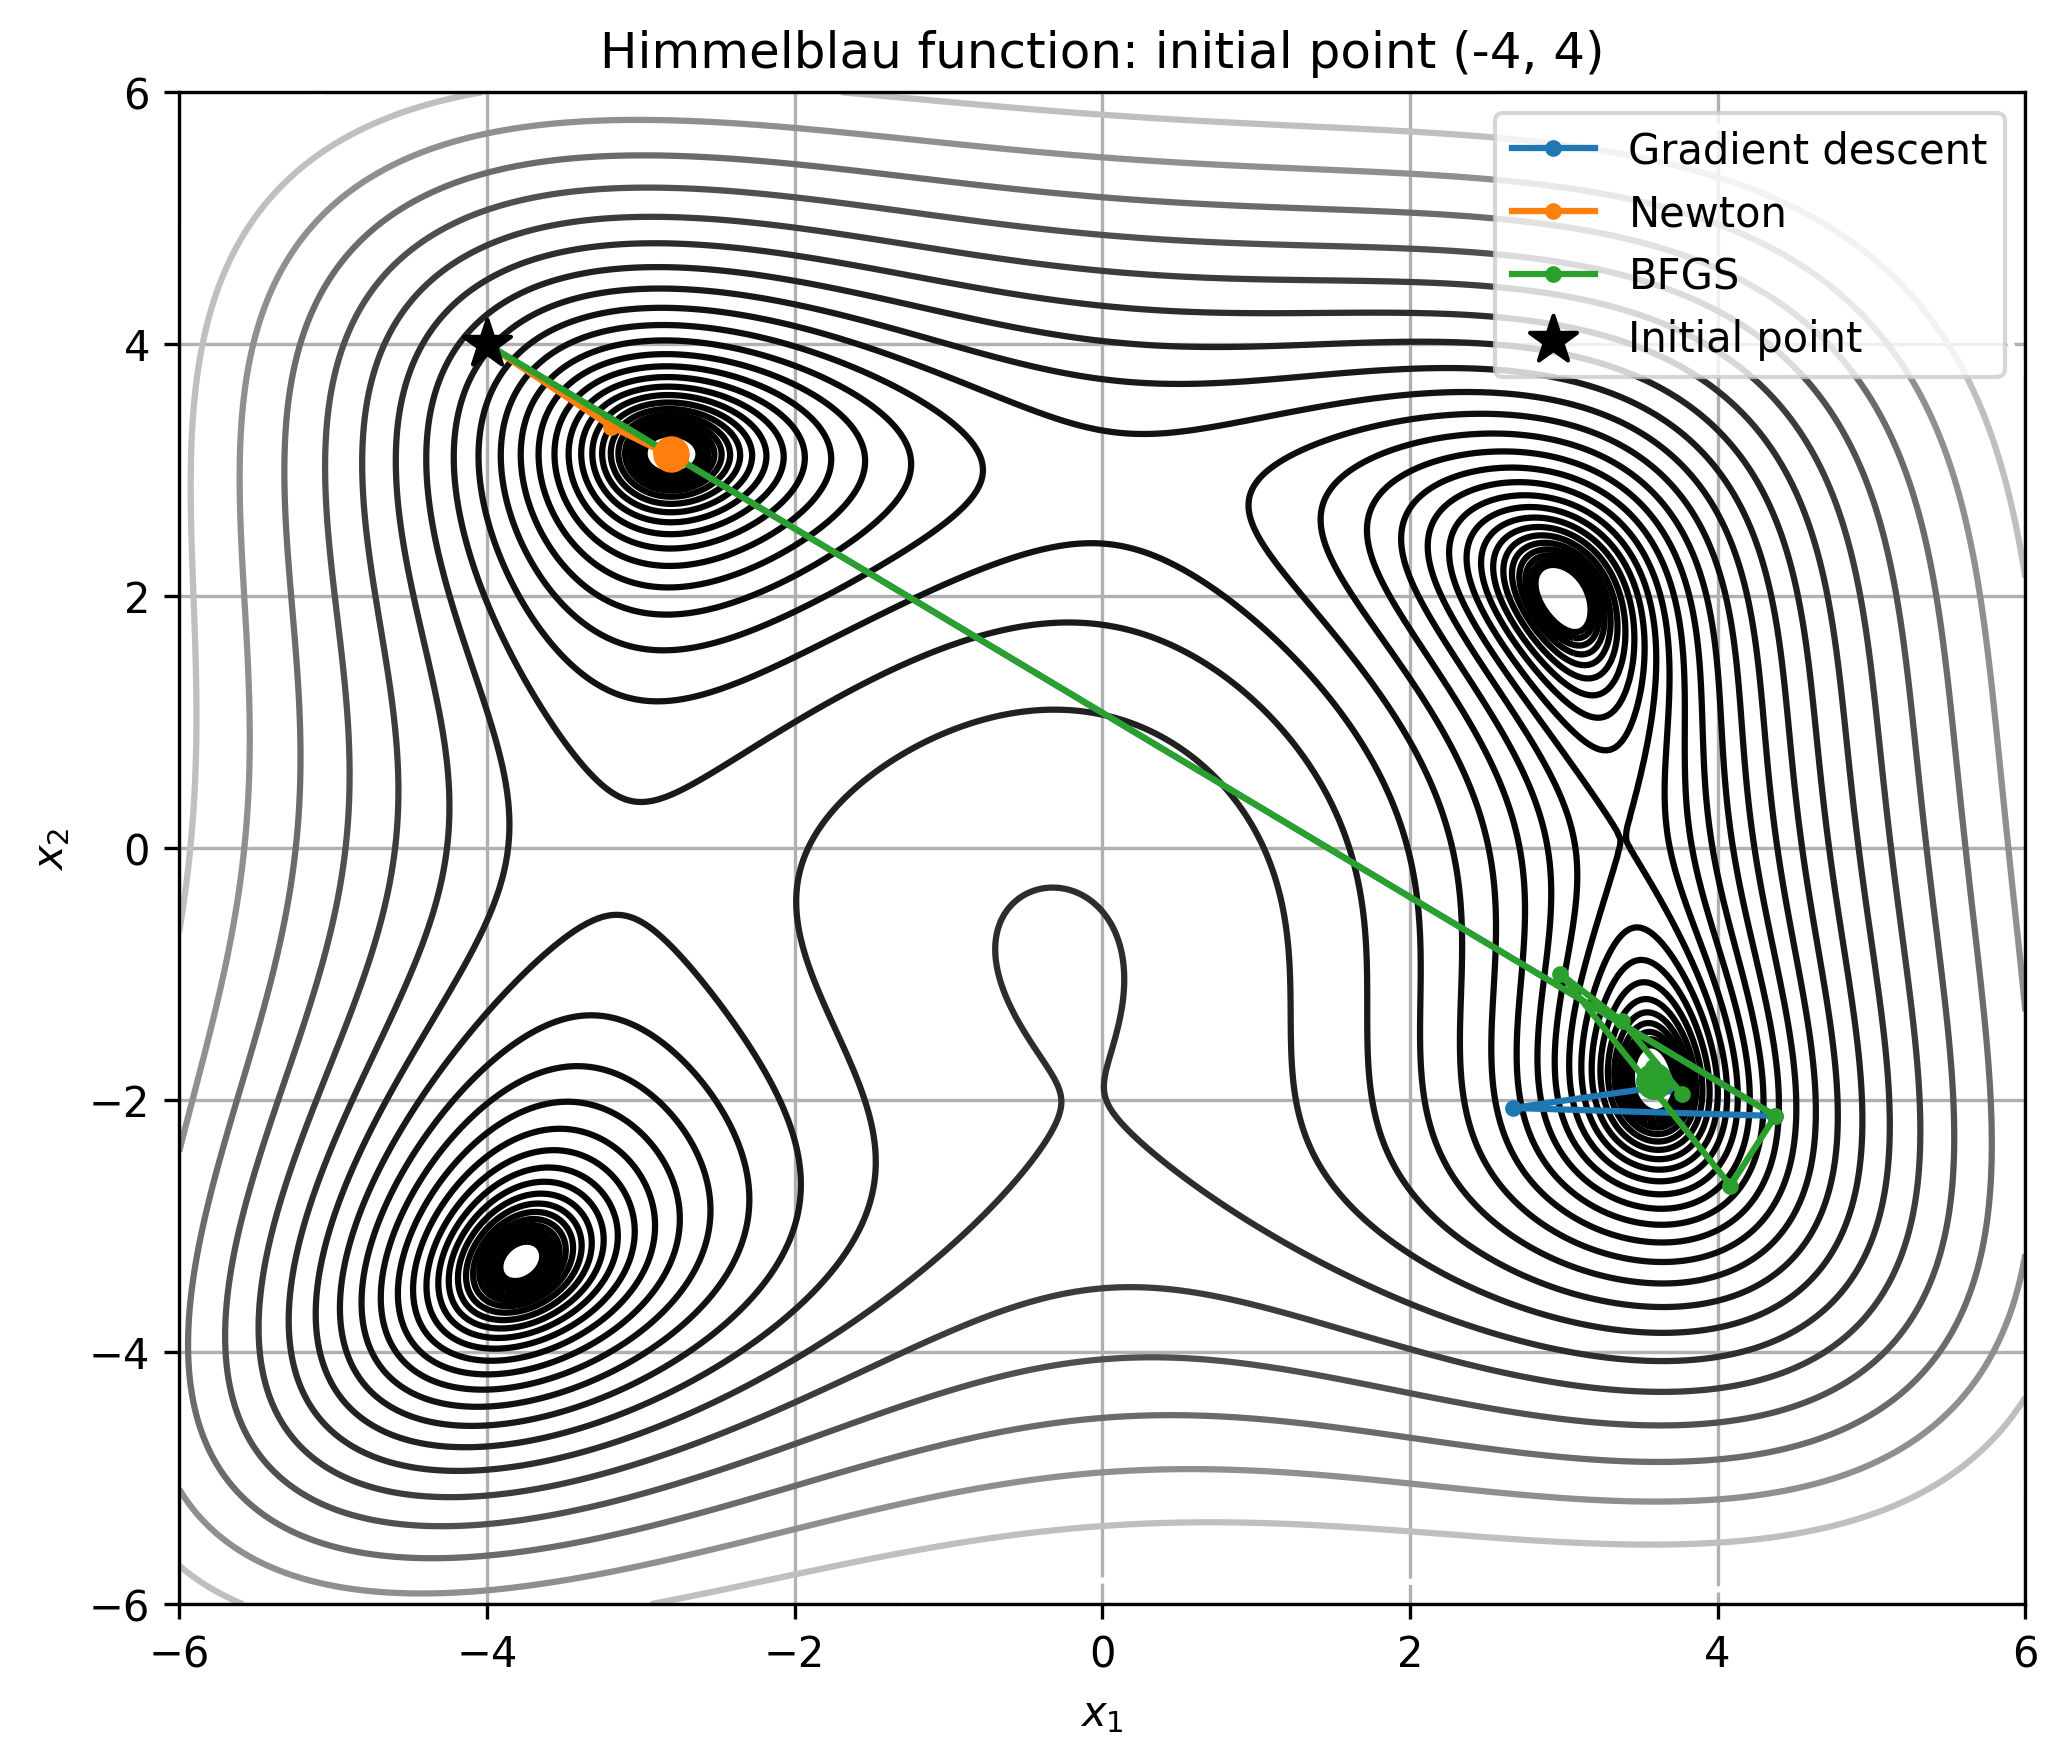
\includegraphics[width=8.5cm]{plots/himmelblau_-4_4.png}
    \caption{初期値 $(-4, 4)$ からの収束経路}
    \label{fig:task2_m4_4}
\end{figure}

\begin{figure}[H]
    \centering
    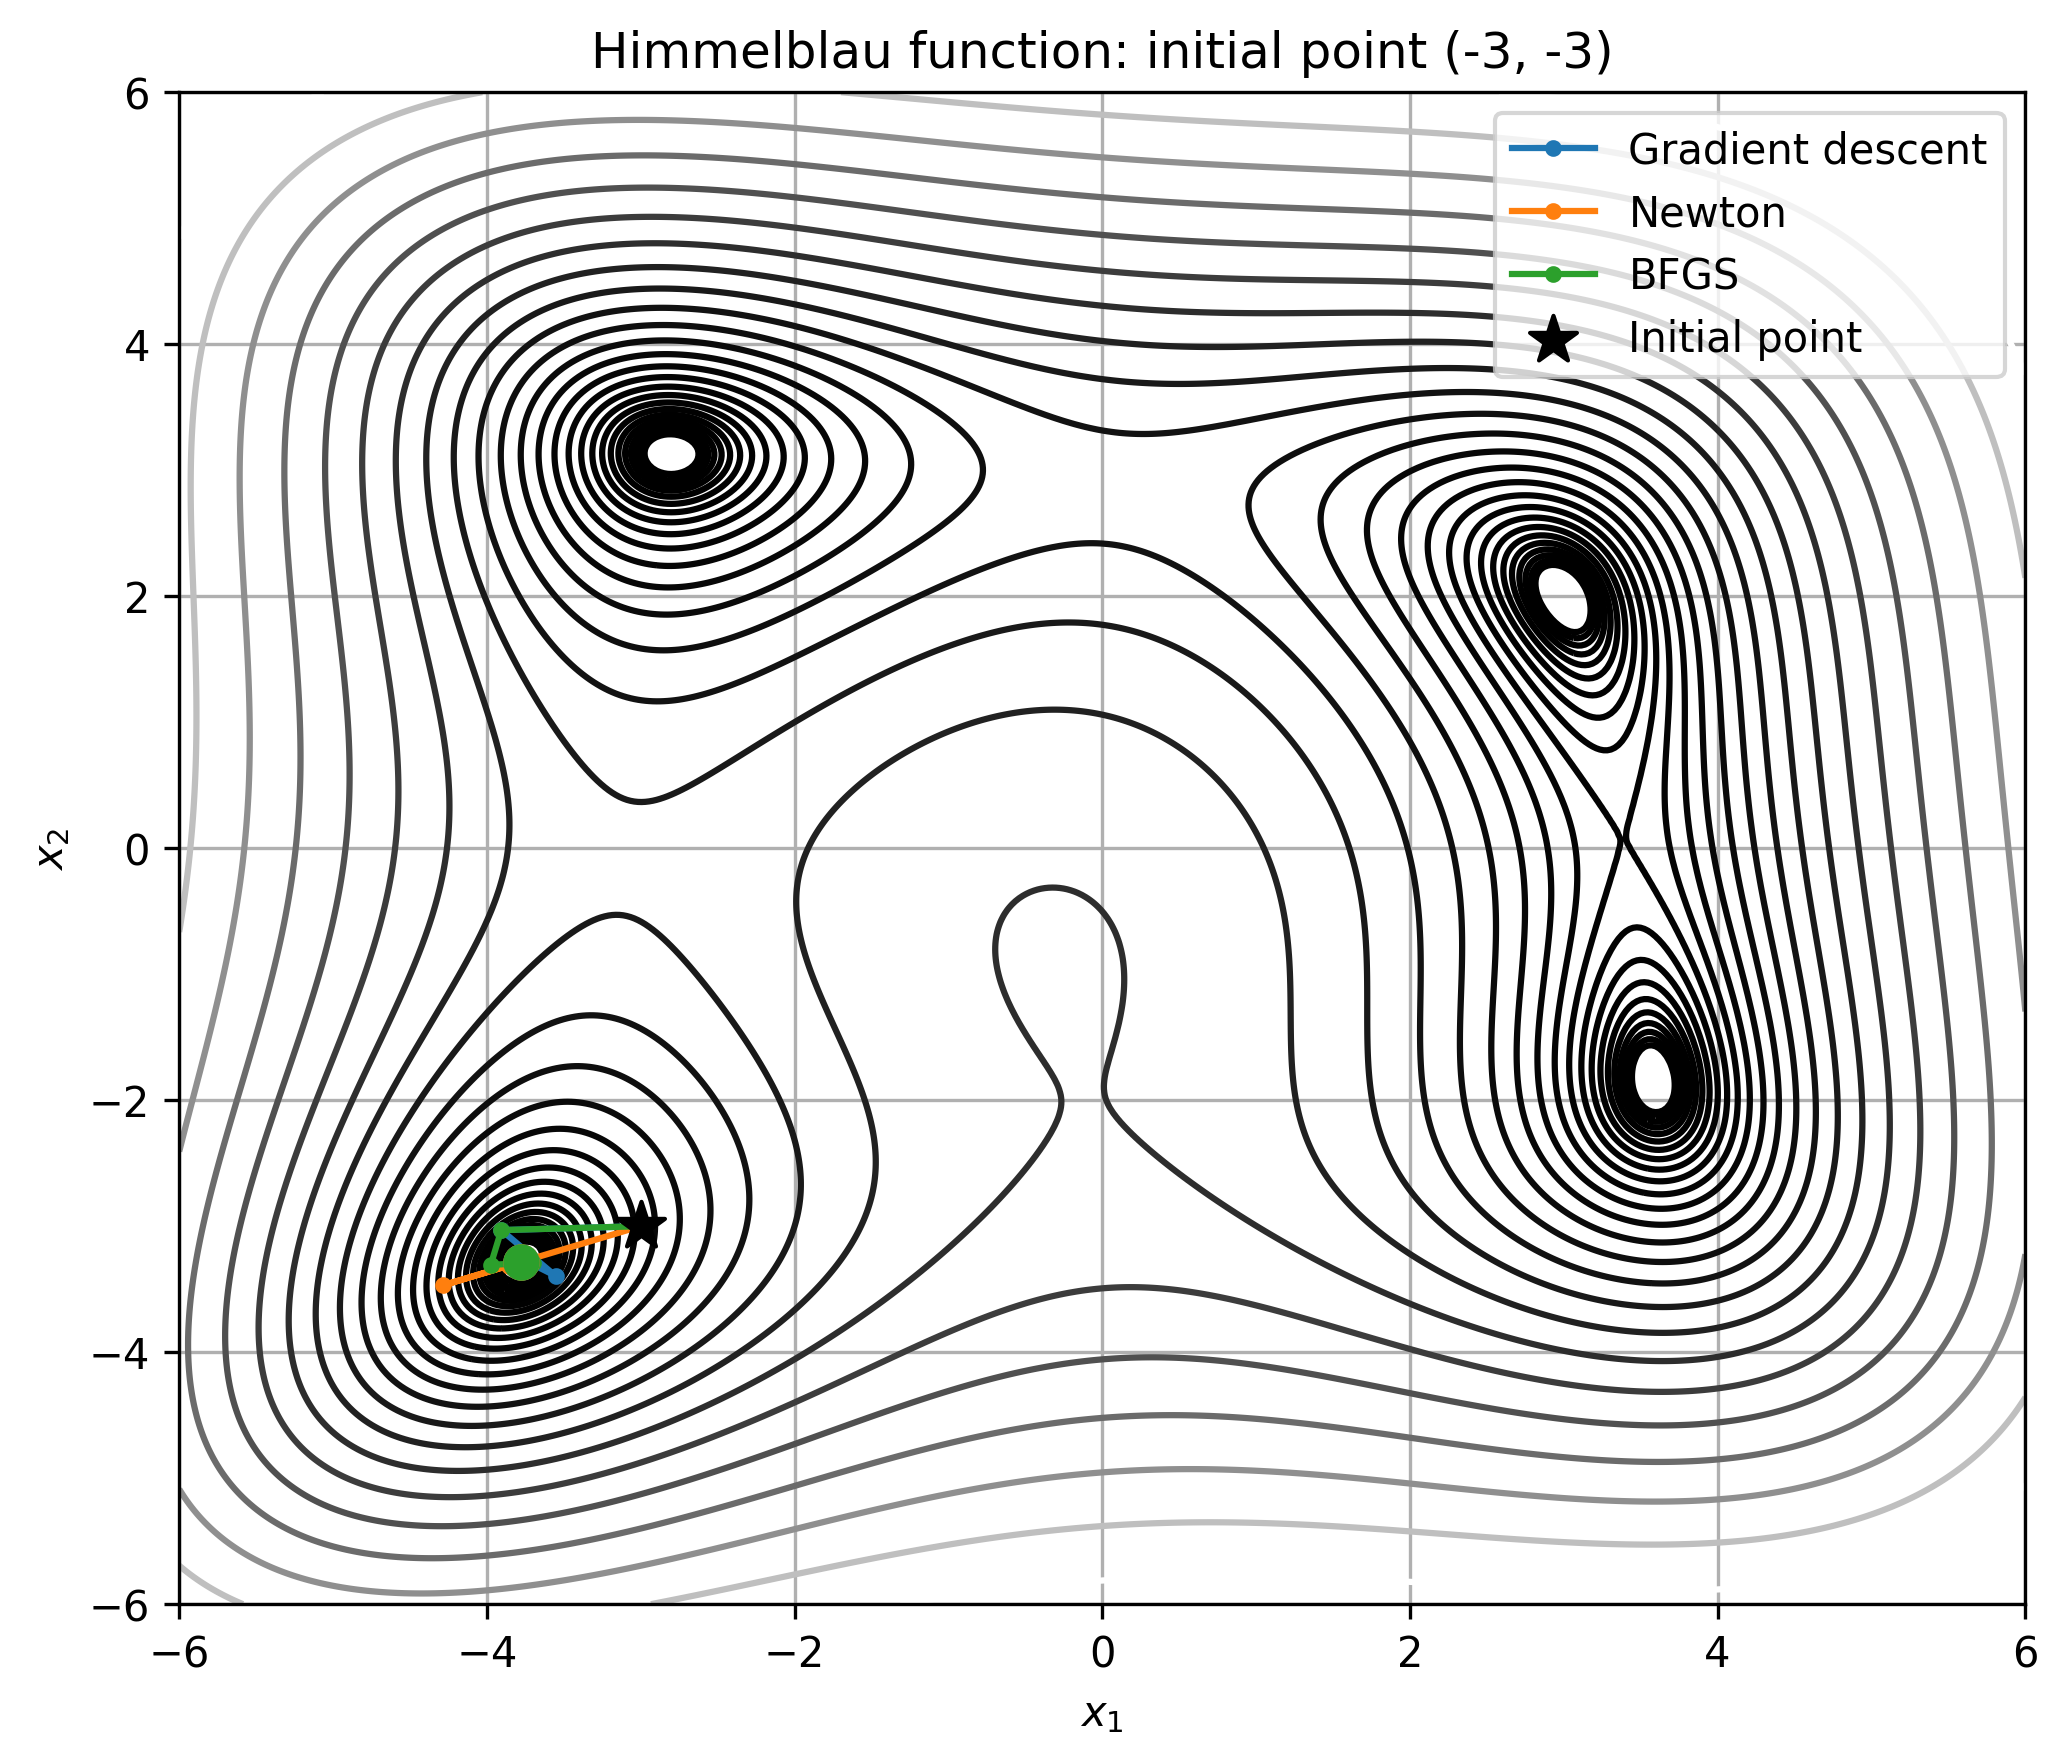
\includegraphics[width=8.5cm]{plots/himmelblau_-3_-3.png}
    \caption{初期値 $(-3, -3)$ からの収束経路}
    \label{fig:task2_m3_m3}
\end{figure}

\begin{figure}[H]
    \centering
    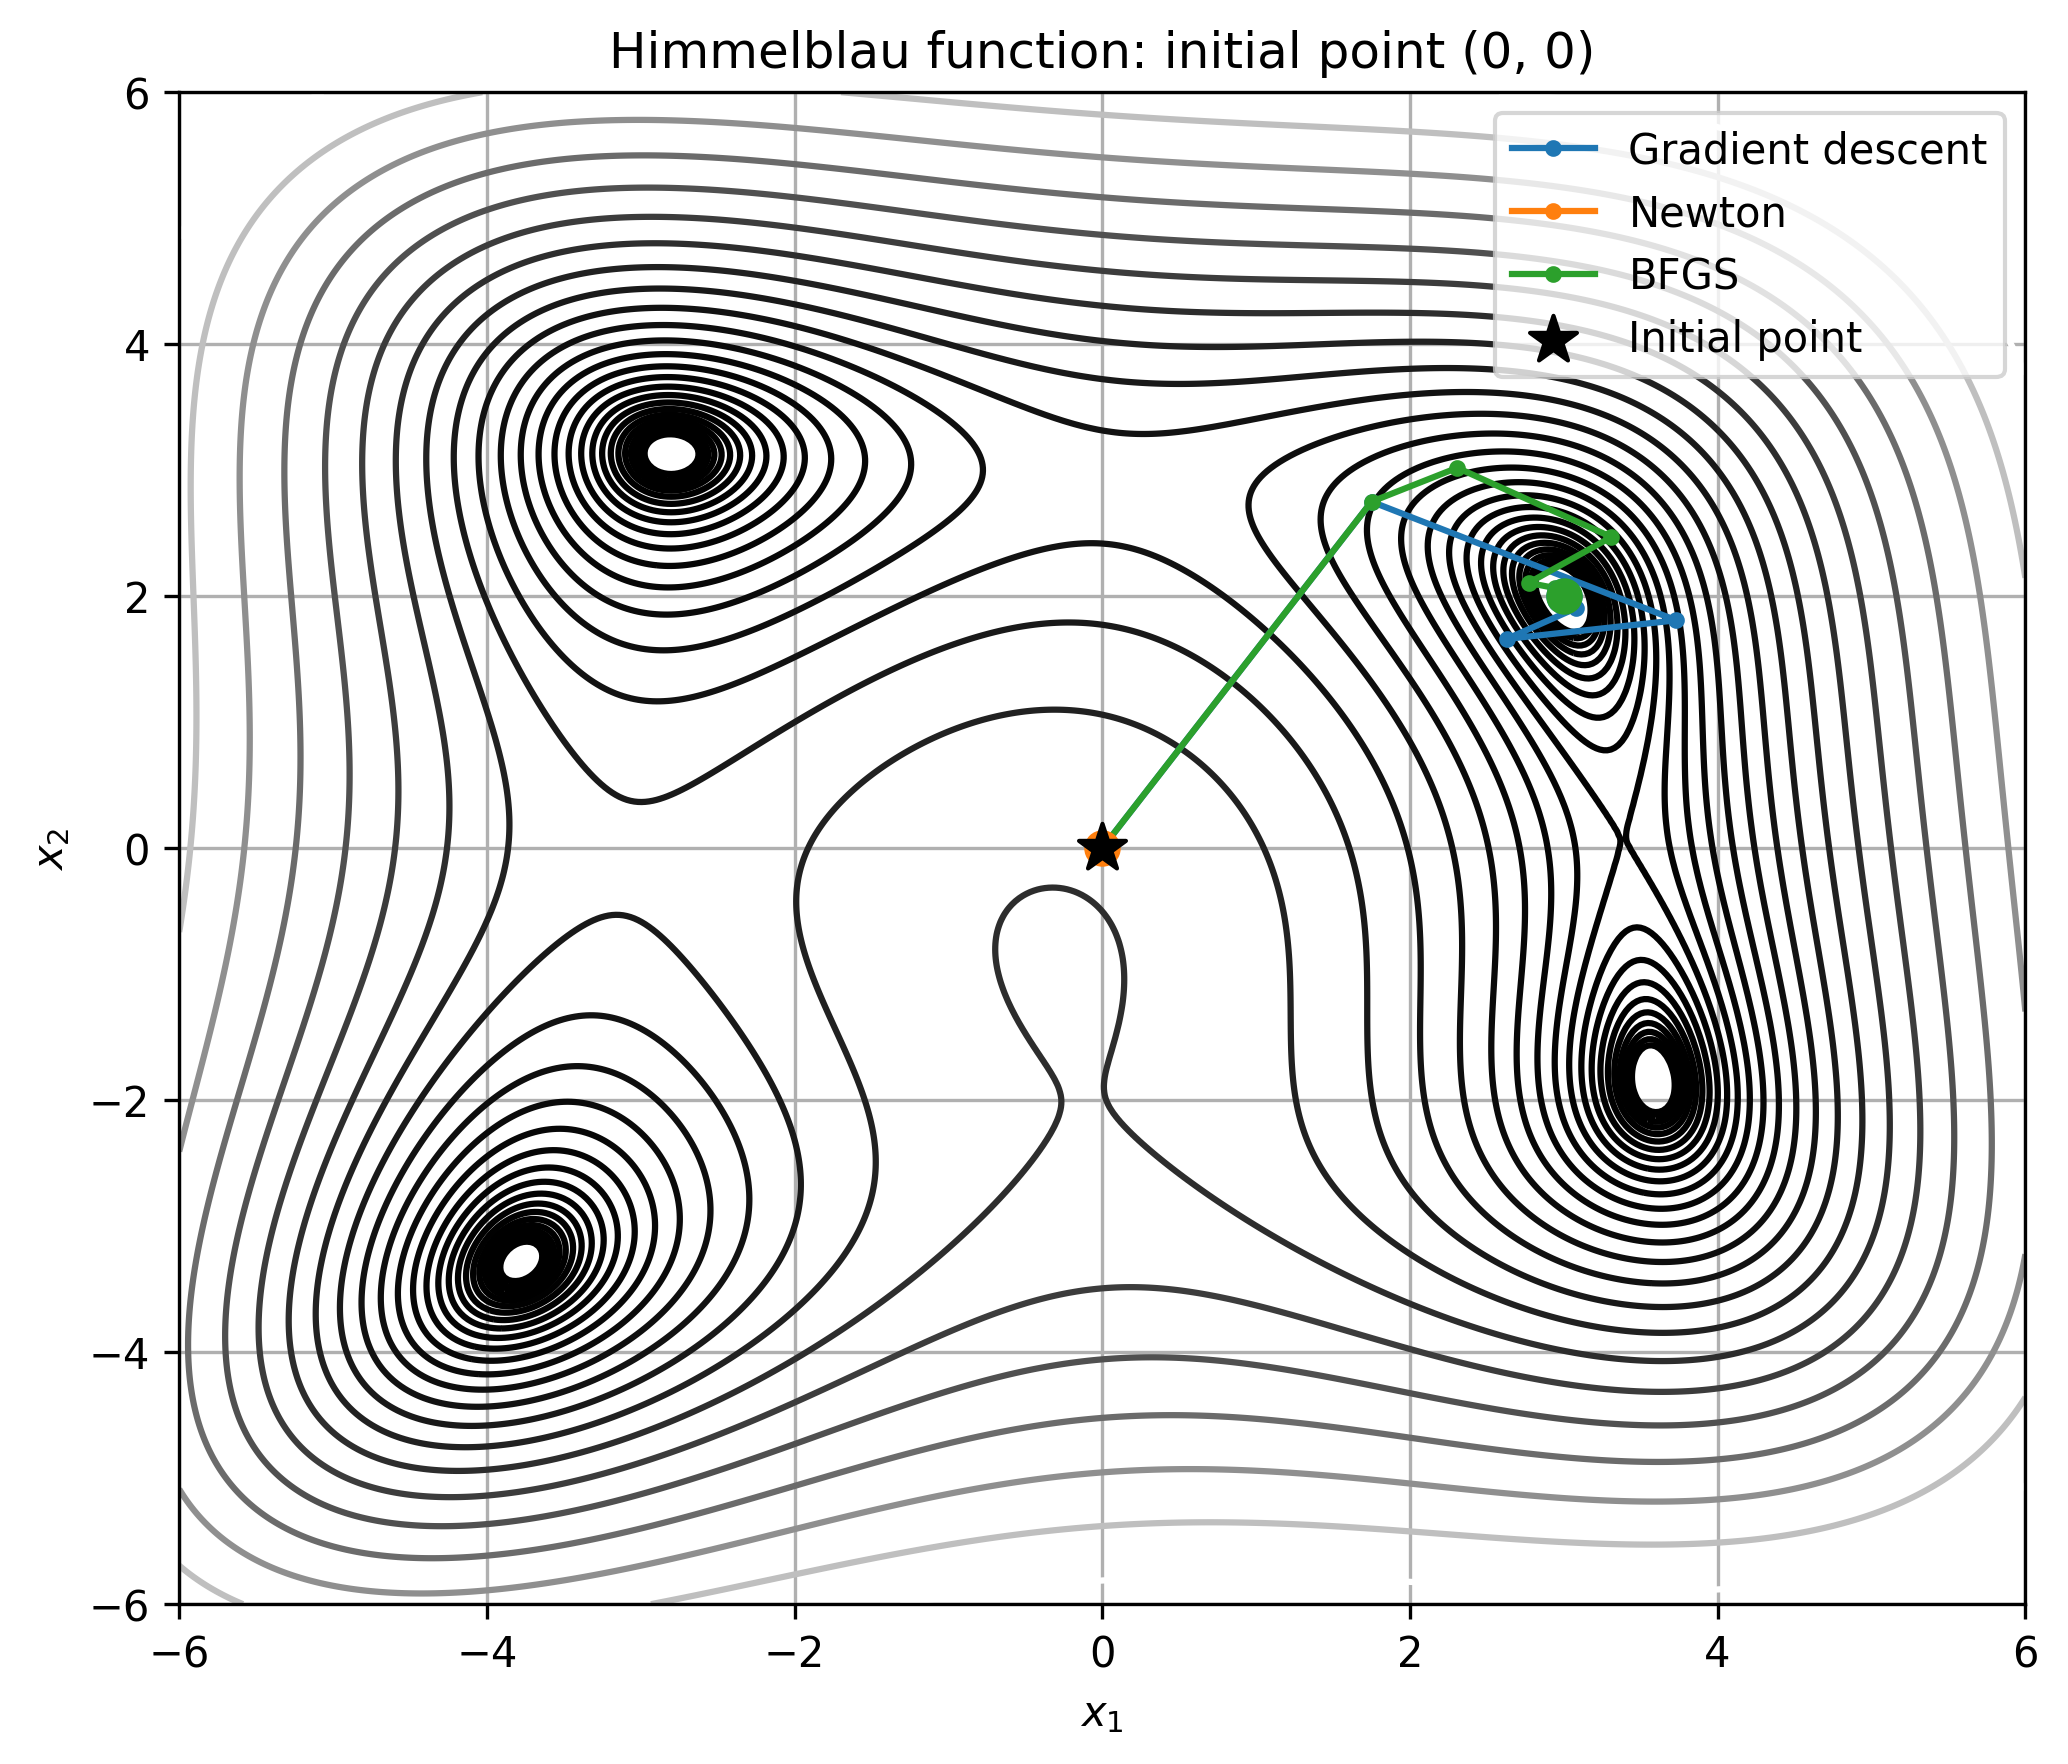
\includegraphics[width=8.5cm]{plots/himmelblau_0_0.png}
    \caption{初期値 $(0, 0)$ からの収束経路}
    \label{fig:task2_0_0}
\end{figure}

\begin{figure}[H]
    \centering
    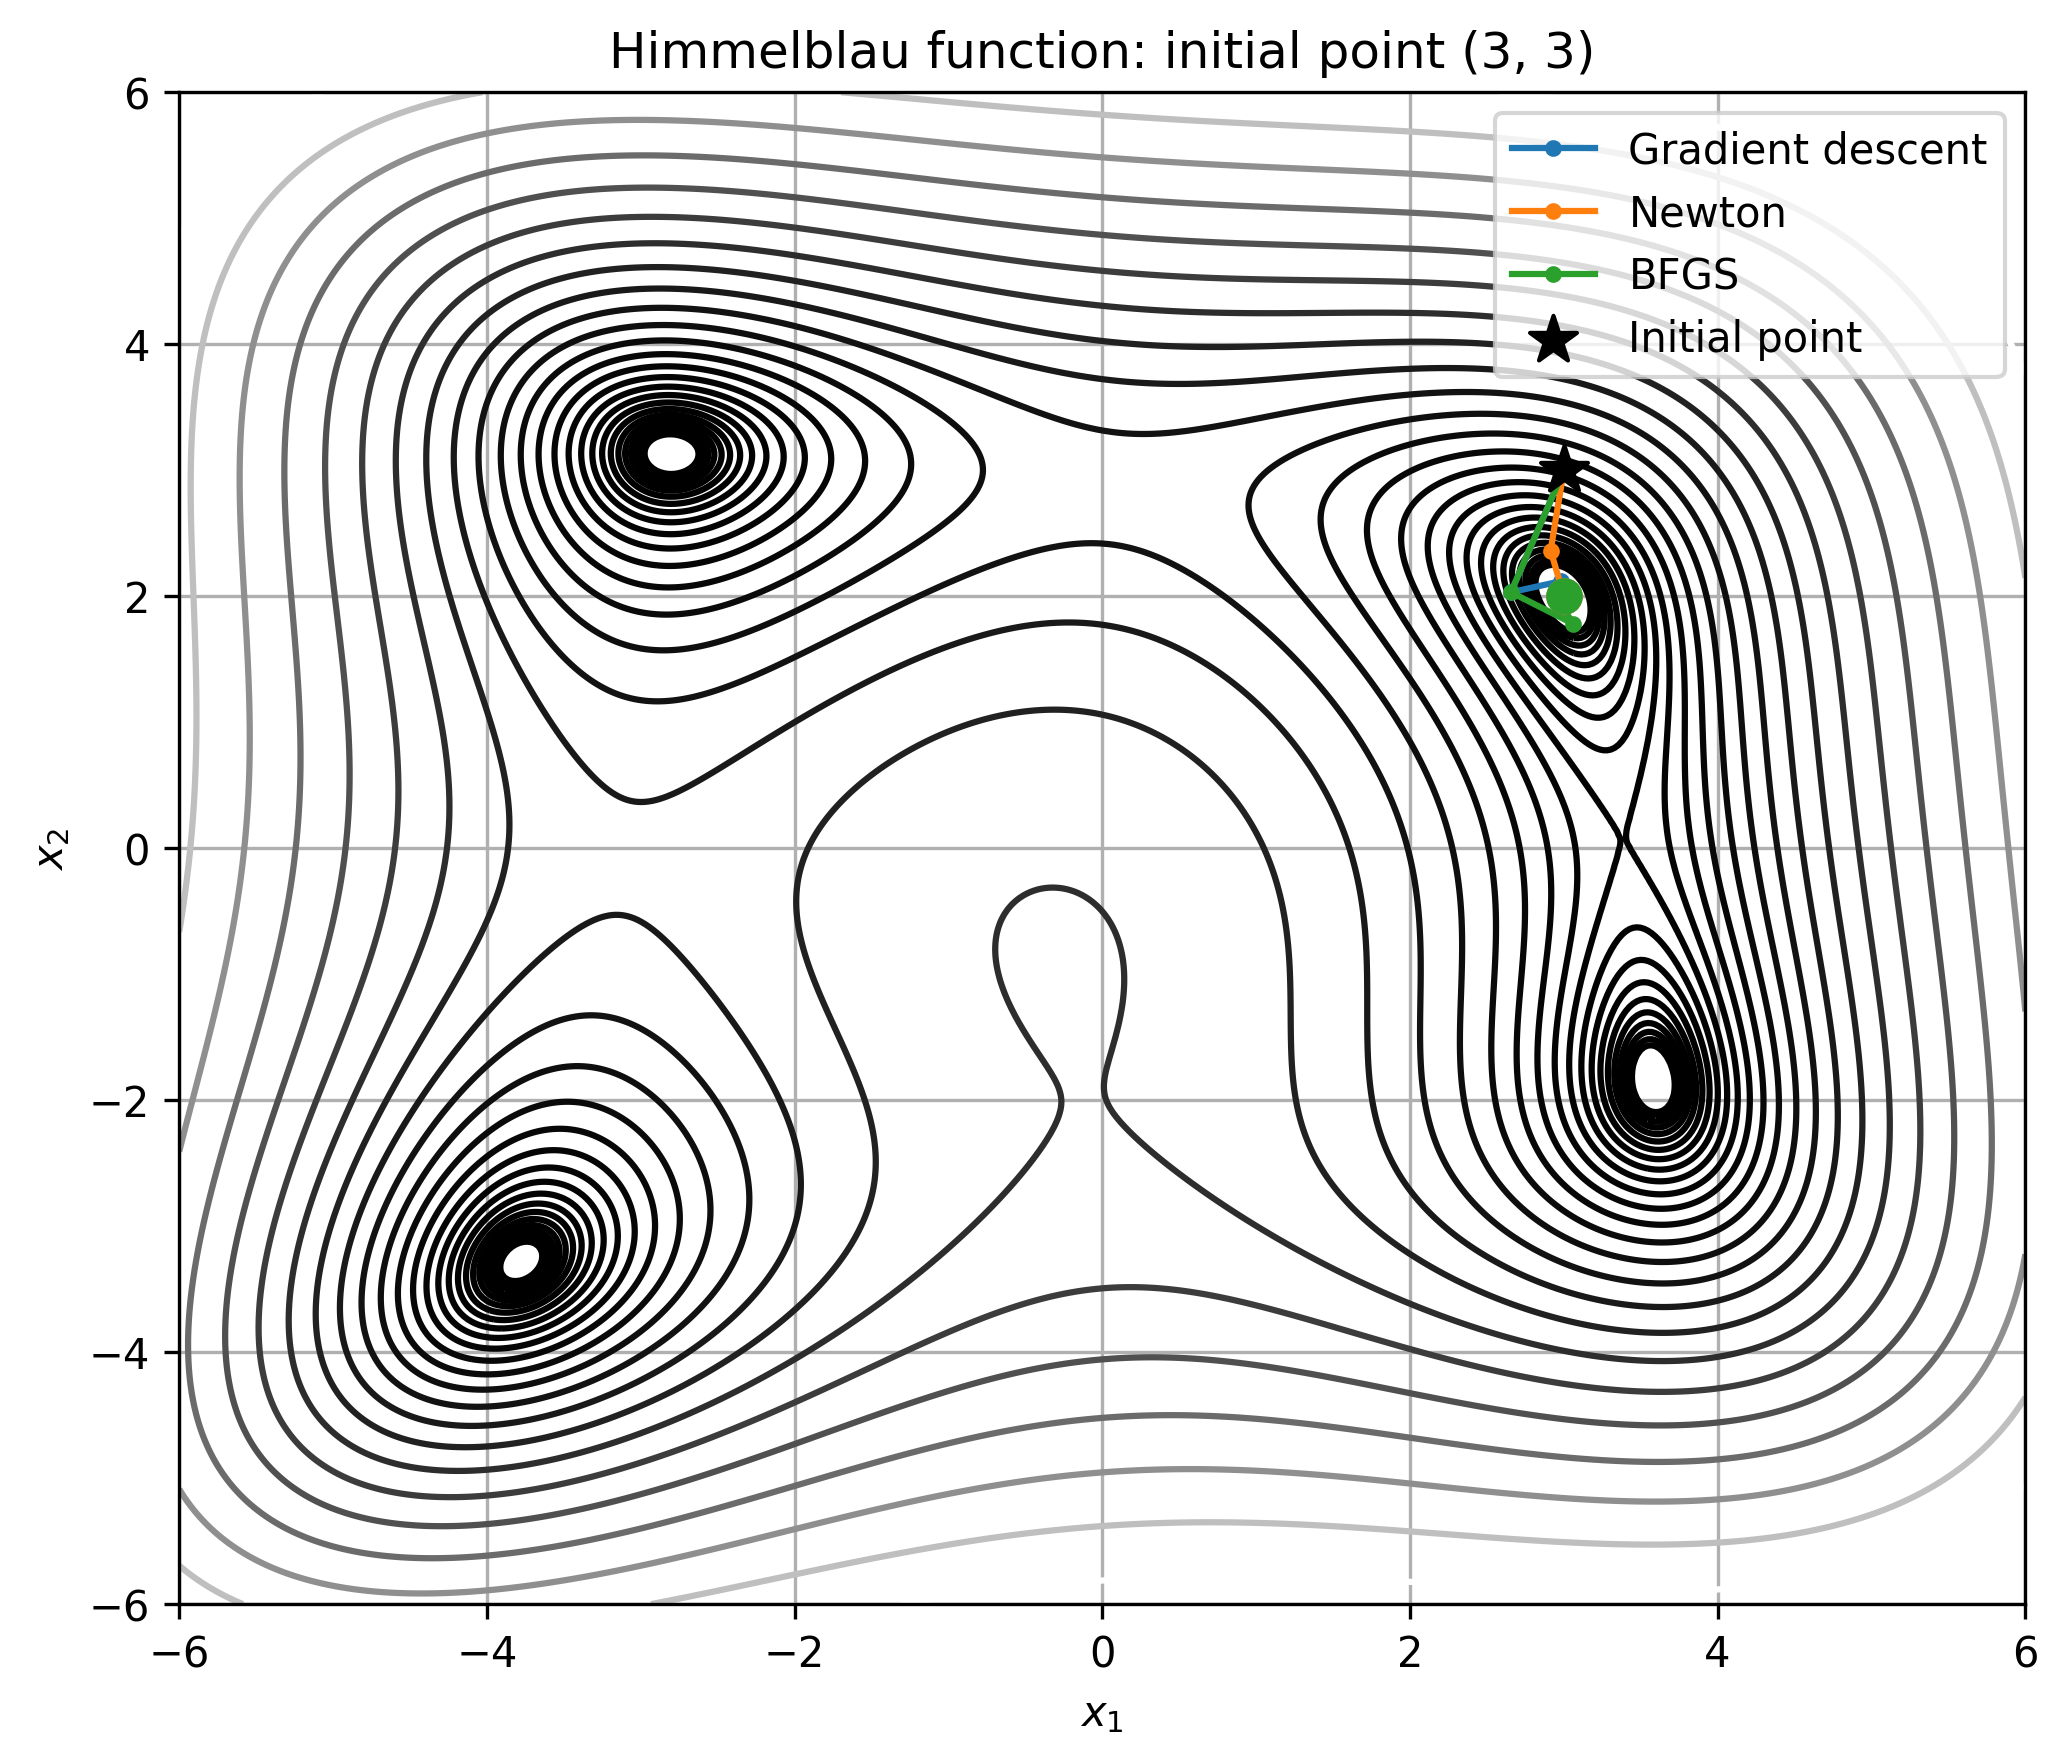
\includegraphics[width=8.5cm]{plots/himmelblau_3_3.png}
    \caption{初期値 $(3, 3)$ からの収束経路}
    \label{fig:task2_3_3}
\end{figure}

\begin{figure}[H]
    \centering
    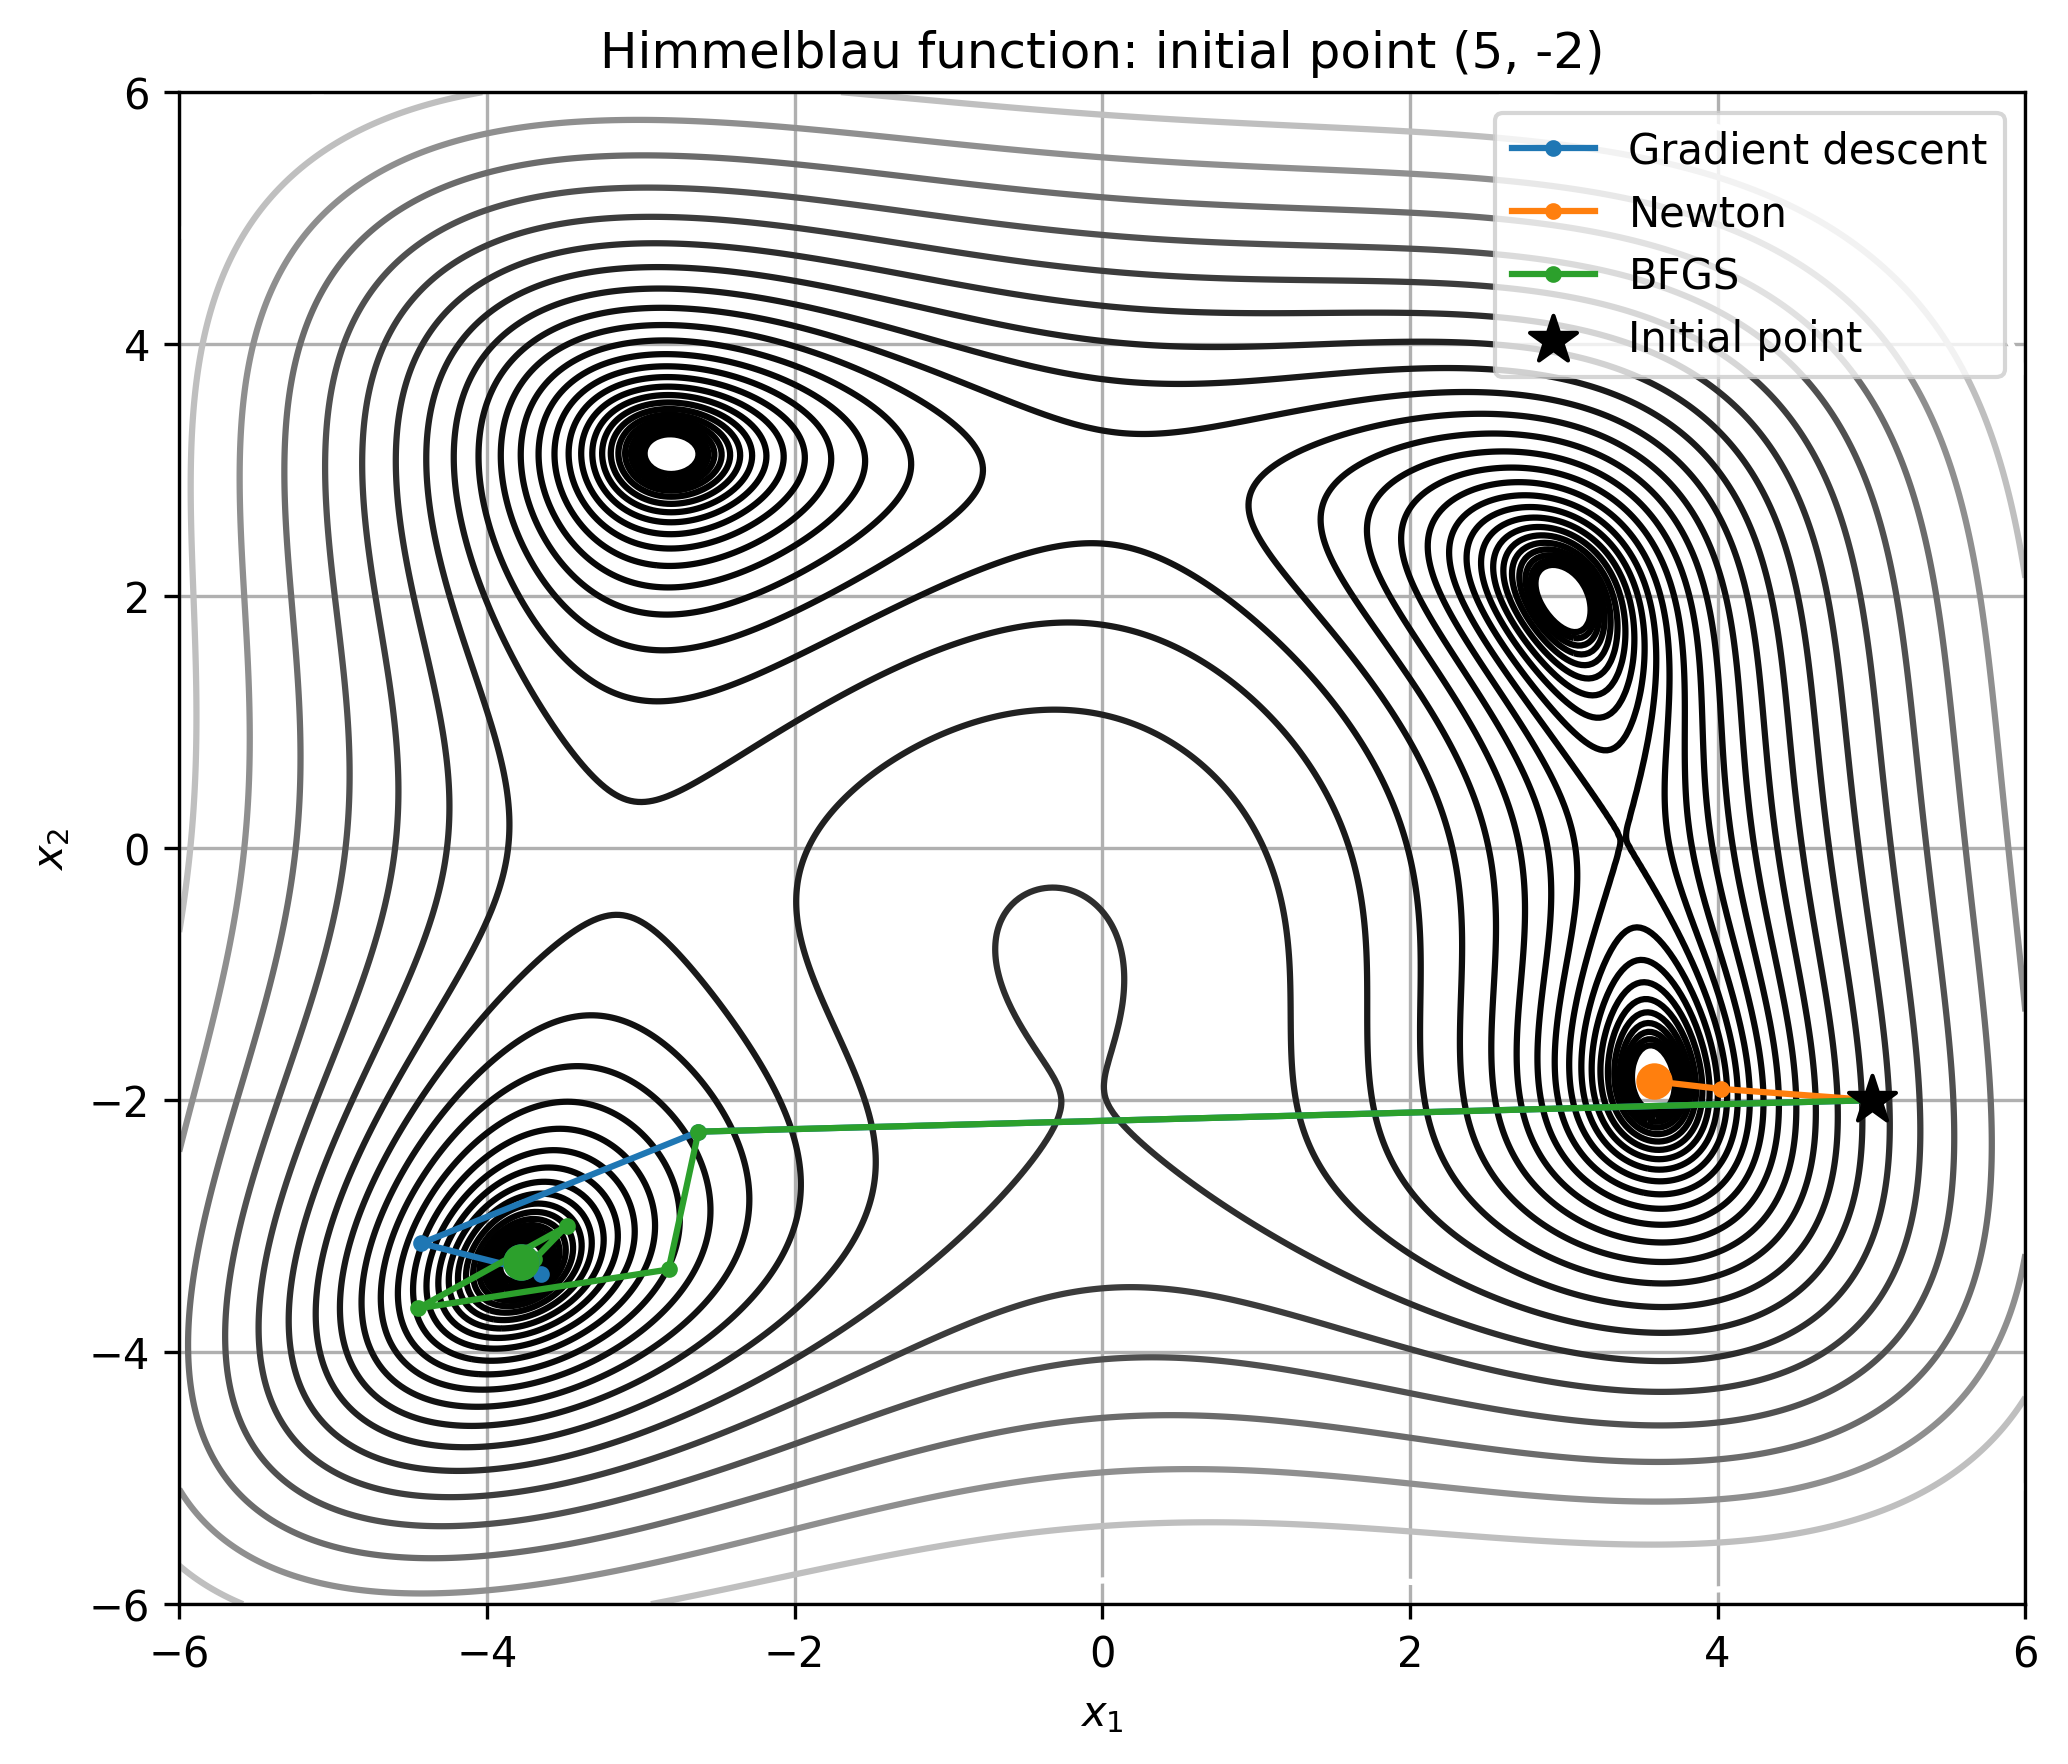
\includegraphics[width=8.5cm]{plots/himmelblau_5_-2.png}
    \caption{初期値 $(5, -2)$ からの収束経路}
    \label{fig:task2_5_m2}
\end{figure}

\subsection{考察}
Himmelblau関数には4つの極小点が存在し、いずれも目的関数値がほぼ0となる大域的最適解である。
しかし、非凸関数であるため、どの解に収束するかは初期値と手法に依存する。
例えば初期値 $(-4,4)$ では、最急降下法とBFGS法は $(3.58,-1.85)$ に収束したのに対し、
Newton法は $(-2.81,3.13)$ に収束した。また、初期値 $(5,-2)$ でも、最急降下法とBFGS法は
$(-3.78,-3.28)$、Newton法は $(3.58,-1.85)$ に収束した。
この結果から、同じ初期値でも更新方向の決め方によって異なる解の吸引領域に入り得ることが分かる。
凸関数では任意の局所解が大域解となり、適切な降下法なら一般に一つの最適解へ向かうのに対し、
非凸関数では複数の局所解が存在し得るため、得られた解が大域解であるかは目的関数値などを比較して判断する必要がある。

Newton法は多くの初期値から5回程度で収束しており、極小点の近傍では二次収束による速さが確認できた。
一方、初期値 $(0,0)$ からは原点付近にとどまり、目的関数値も170のまま最大反復回数100回に達した。
したがって、この場合は勾配ノルムによる収束ではなく未収束である。Newton方向
$d_k=-\{\nabla^2 f(x_k)\}^{-1}\nabla f(x_k)$ はHesse行列が正定値なら降下方向となるが、
非凸領域ではHesse行列が不定または負定値となり、必ずしも $\nabla f(x_k)^{\mathsf T}d_k<0$ を満たさない。
このような方向に通常のArmijo型バックトラッキングを適用しても、十分な降下が得られず停滞する場合がある。

3手法ともバックトラッキング直線探索を用いているが、安定性には探索方向の性質による差が見られた。
最急降下方向は常に降下方向であり、BFGS法も正定値な初期近似から始め、
$s_k^{\mathsf T}y_k>0$ を満たす場合に更新することで近似Hesse行列の正定値性を保ちやすく、
今回の全初期値で目的関数値がほぼ0の極小点へ収束した。一方、Newton方向は非凸領域では降下方向とは限らないため、
バックトラッキングを用いても極小点への収束が保証されない。BFGS法は最急降下法より少ない反復回数で収束したが、
これらの手法でも初期値によって異なる大域解に収束しており、
一つの初期値だけでは他の解を発見できない。

Newton法を非凸問題で安定化するには、Newton方向が降下方向であるかを確認し、そうでなければ負の勾配方向へ切り替える方法、
Hesse行列に正の対角成分を加えて正定値化する修正Newton法、直線探索や信頼領域法などが有効である。
また、複数の初期値から計算するマルチスタートを用い、得られた停留点の目的関数値と二次の最適性条件を比較することで、
局所解への依存を減らし、大域解を探索する必要がある。

\section{課題3: KKT条件を「有効制約集合」で実装する}
目的関数: $\min f(x)=(x_{1}-a)^{2}+(x_{2}-b)^{2}$ \\
制約条件: $g_{1}=x_{1}^{2}+x_{2}^{2}-1 \le 0,\ g_{2}=-x_{1} \le 0,\ g_{3}=-x_{2} \le 0$

\subsection{各中心点における最適解と有効制約}
4つの異なる中心点 $(a,b)$ に対してActive-set法を実行した結果を以下の表に示す。中心点の位置によって、最終的にどの制約が有効（Active）になるかが変化していることがわかる。

\begin{table}[hbtp]
    \centering
    \caption{各中心点に対する最適解と有効制約・乗数の結果}
    \begin{tabular}{lcccc}
        \toprule
        中心点 $(a,b)$ & 最適解 $x^*$ & 目的関数値 $f(x^*)$ & 有効制約 $A^*$ & 乗数 $\mu^*$ \\
        \midrule
        $(2, 1)$   & $(0.8944, 0.4472)$ & $1.5279$ & $\{g_1\}$ & $(1.2361, 0, 0)$ \\
        $(-1, 1)$  & $(0, 1)$           & $1.0000$ & $\{g_2\}$ & $(0, 2, 0)$ \\
        $(1, -1)$  & $(1, 0)$           & $1.0000$ & $\{g_3\}$ & $(0, 0, 2)$ \\
        $(-1, -1)$ & $(0, 0)$           & $2.0000$ & $\{g_2, g_3\}$ & $(0, 2, 2)$ \\
        \bottomrule
    \end{tabular}
\end{table}

\subsection{KKT解の判定チェックリスト（抜粋）}
アルゴリズム内部でKKT条件がどのように検証されているかを示すため、中心点 $(a,b) = (2,1)$ において、いくつかの有効制約を仮定した際の判定チェックリストを抜粋して以下に示す。

\begin{table}[hbtp]
    \centering
    \caption{中心点 $(2,1)$ におけるKKT解の判定チェックリスト}
    \begin{tabular}{ccccccc}
        \toprule
        仮定した $A$ & 1.主実行 & 2.有効整合 & 3.無効整合 & 4.双対実行 & 5.相補性 & 総合判定 \\
        \midrule
        $\{\phi\}$  & NG & OK & OK & OK & OK & 不適合 \\
        $\{g_2\}$   & OK & OK & OK & NG & OK & 不適合 \\
        $\mathbf{\{g_1\}}$ & \textbf{OK} & \textbf{OK} & \textbf{OK} & \textbf{OK} & \textbf{OK} & \textbf{KKT条件クリア} \\
        \bottomrule
    \end{tabular}
\end{table}

\subsection{考察}
本問は、中心点 $(a,b)$ を第一象限の単位円内へ射影する問題と解釈できる。
そのため、$(2,1)$ では円周の $g_1$、$(-1,1)$ では $y$軸の $g_2$、
$(1,-1)$ では $x$軸の $g_3$、$(-1,-1)$ では両軸の $g_2,g_3$ が有効となった。
中心点の位置と有効制約の変化は、幾何学的な予想と一致している。

乗数 $\mu_i$ は、目的関数の勾配を制約境界で押し返す力の大きさと解釈できる。
実際に解を境界へ押し留める制約では乗数が正となり、解に影響しない制約では0となった。
また、中心点 $(2,1)$ では、有効制約なしの場合は主実行可能性を満たさず、
$g_2$ を仮定した場合は乗数が負となって双対実行可能性を満たさなかった。
一方、$g_1$ を仮定すると全KKT条件を満たしたことから、Active-set法によって正しい有効制約を選択できたといえる。

なお、中心点 $(-1,1)$ では $\{g_2\}$ と $\{g_1,g_2\}$、$(1,-1)$ では
$\{g_3\}$ と $\{g_1,g_3\}$ の2通りがKKT条件を満たし、同じ最適解と目的関数値を与えた。
これは円制約 $g_1$ も等号を満たす一方、その乗数が0で解に影響しないためである。
現在の実装は目的関数値が最小の候補を選び、値が同じ場合は列挙順で先の候補を採用するため、
表ではそれぞれ $\{g_2\}$ と $\{g_3\}$ が表示されている。
\appendix
\section{実装した関数一式}
課題1から課題3で使用した主要な関数を以下に示す。
\lstinputlisting[
    language=Python,
    caption={課題1--3で使用した関数一式},
    basicstyle=\ttfamily\scriptsize,
    breaklines=true,
    numbers=left,
    numberstyle=\tiny
]{kadai1_appendix.py}

\end{document}
